\centering
\begin{columns}[totalwidth=.9\textwidth]
    \column{.6\textwidth}
            \begin{itemize}
                \item 連結性を不均一に
                    \begin{itemize}
                        \item 連結に\alert{位置依存性}
                    \end{itemize}
                \item 巨視的な変形後
                    \begin{itemize}
                        \item 結節点のゆらぎが不均一
                        \item 多様な緩和モード
                        \item \alert{緩和の長時間化?}
                    % \item ファントムネットワークモデルの諸特性の発現?
                    \end{itemize}
                \item \alert{解析を容易}に、
                    \begin{itemize}
                        \item 既往研究で反応系
                        \item ストランド長と結合数を一定
                    \end{itemize}
            \end{itemize}
    \column{.35\textwidth}
        ランダム構造の模式図
        \vspace{10mm}
        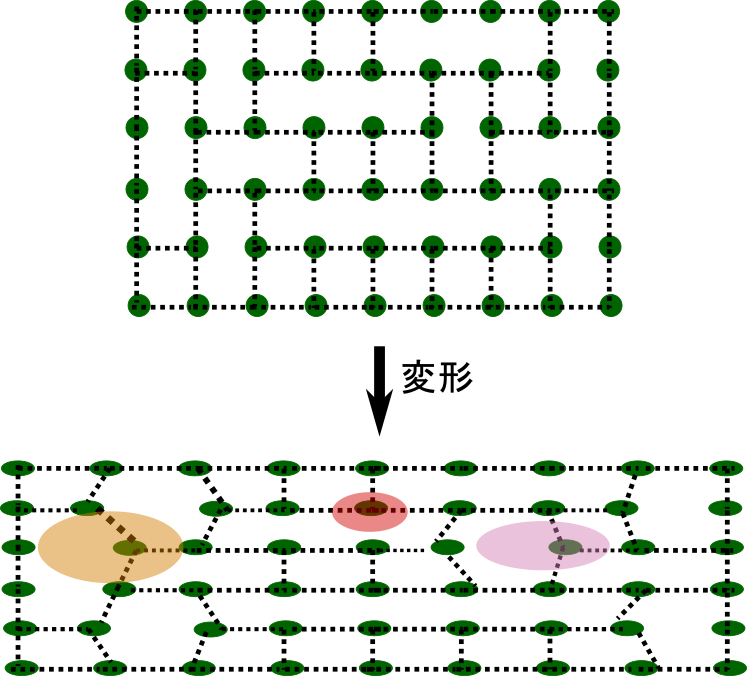
\includegraphics[width=\textwidth]{random_NW.png}
\end{columns}